% !TEX encoding = UTF-8 Unicode

\documentclass[a4paper]{article}
\usepackage{subfigure}
\usepackage{wrapfig}
\usepackage{caption}
\usepackage{color}
\usepackage{url}
\usepackage{amsthm}
\usepackage{amsmath}
\usepackage[utf8]{inputenc} % čudni karakteri
\usepackage{graphicx}
\usepackage[english, serbian]{babel}
\usepackage[unicode]{hyperref}
\hypersetup{colorlinks,citecolor=green,filecolor=green,linkcolor=blue,urlcolor=blue}

\begin{document}

\title{Rubikova kocka\\ \small{Seminarski rad u okviru kursa\\Tehničko i naučno pisanje\\ Matematički fakultet}}

\author{Jovana Brkljač\\ bjovana314@gmail.com \and Mateja Janić\\ janic.mateja@gmail.com \and Bogdan Pejčić \\ bogdan.pejcic@gmail.com \and Mitar Avramović \\ 59.16.16.10.ma@gmail.com}
\date{15.~novembar 2022.}
\maketitle

\abstract{
U ovom radu je ukratko i pojednostavljeno prikazan istorijat Rubikove kocke, ali i načini njenog funkcionisanja i rešavanja. Potrebno je naglasiti da sami algoritmi za rešavanje Rubikove kocke mogu biti veoma komplikovani za razumevanje i zahtevaju puno dokaza i teorema, koje ovde nije bilo moguće izložiti. 
}
\tableofcontents

\newpage

\section{Uvod i istorijat}
\label{sec:uvod}

\setlength{\parindent}{25pt}
\vspace{0.4cm}
Godina je 1974. i na Fakultetu primenjenih umetnosti u Budimpešti, jedan profesore pokušava, prema njegovim rečima, da napravi zanimljiv zadatak za svoje studente. Naime, Erne Rubik\footnote{{Ernő Rubik (1944 - )}} je osmislio drvenu strukturu u obliku kocke, čiji delovi bi mogli da se nezavisno pomeraju a da sama struktura ostane sastavljena. \\*
\hspace{3ex}Kada je shvatio šta je zapravo napravio, izum je patentirao i pokrenuo marketing kampanju. Tako je prva ,,Magična kocka'' polako krenula da osvaja svet i srca matematičara svih uzrasta.\\*
\hspace{15pt}Zbog svoje specifičnosti i (naizgled) jednostavnosti, ova ,,igračka'' je od samog početka izazvala veliku buru u javnosti. Krenula su mnogobrojna takmičenja u sastavljanju kocke, gde je težnja bila da se ona sastavi u što kraćem vremenskom roku. Iako su se već tada pojavljivali ljudi koji su mogli da je sastave u vremenu manjem od minut, Rubikova kocka se već tada ustoličila kao jedan od ozbiljnijih problema matematičarima, zbog složenosti do koje dolazi nakon samo nekoliko poteza i izraženih algebarskih osobina. \\

Tada, ispred najvećih matematičkih umova, su se postavila dva pitanja. Prvo je bilo ,,Da li postoji algoritam po kome bi se kocka mogla sastaviti?'' a drugo je bilo ,,Za koliko najmanje poteza je moguće sastaviti Rubikovu kocku (nezavisno od početne pozicije)?'' Takav broj poteza je dobio naziv \textit{Božji broj} a potencijalni algoritam koji bi nas doveo do optimalnog stanja \textit{Božji algoritam}\footnote{termin Božji algoritam se odnosi i na druge matematičke slagalice (npr. Hanojska kula), ali je prvobitno bio korišćen za problem Rubikove kocke}. Paralaleno sa nastankom Rubikove kocke dolazi i do ubrzanog razvoja računara, te su i oni bili upošljeni u potrazi za brojem i algoritmom. Ovo je bio jedan od prvih ozbiljnijih primera čovekove potrage za rešenje matematičkog problema pomoću računara. \\

Inicijalni problem u potrazi je bio taj što je postojao preveliki broj mogućih početnih stanja u kojima se kocka može naći. Značajne pomake ka postizanju tog cilja su napravili Morven Tisltvejt\footnote{{Morwen Thistlethwaite}, britanski matematičar}, Herbert Kosiemba\footnote{{Herbert Kociemba} (1954 - ), nemački nastavnik matematike} i Ričard Korf\footnote{{Richard Korf}, američki programer i profesor} čiji su algoritmi promenili način sagledavanja kocke i načine na koji će se rešenje tražiti.\\*
Prve procene donje granice izlaze vrlo brzo, gde se 18 pominje kao moguć broj. Mada se tek 1995. definitivno pokazuje da je donja granica 20 poteza. Sa druge strane, prva procena gornje granice se javlja 1979. godine i postavlja se na 277 poteza. Kasnije se, pomoću gorenavedena tri algoritma, taj broj smanjiti i doći do aktuelne gornje granice od svega 30 poteza.  \\

U 21. veku se, zbog sve većih mogućnosti računara, stavlja sve veći i veći akcenat na što boljoj optimiziaciji i smanjenju velikog broja slučajeva. Tako u julu 2010. godine tim istraživača (među kojima je bio i Koisemba) uspeva da dođe do samog Božjeg broja. Uspeli su da dokažu da je to 20 poteza.

\section{Elementi Rubikove kocke}
\label{sec:elementi}

    \begin{wrapfigure}{r}{3cm}
         \centering
         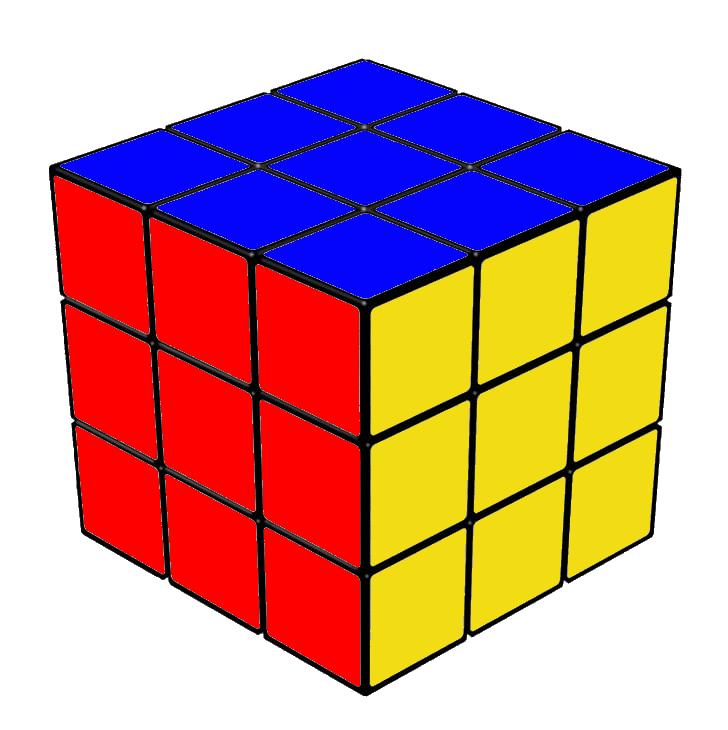
\includegraphics[width=2.5cm]{images/slozena-kocka.png} 
         \caption{}
         \label{fig:kocka}
    \end{wrapfigure}

Rubikova kocka je struktura u obliku kocke kojoj je svaka od strana podeljena na 9 manjih kvadrata, što stvara sliku kao da se sastoji od $3^3 = 27$ manjih kocki (slika \ref{fig:kocka}).
Svaka od strana kocke je obojena jednom bojom i cilj je rasturenu kocku vratiti u početni položaj. Početni položaj kocke je podrazumevano položaj kao na slici (slika \ref{fig:kocka})

U samom centru kocke se ne nalazi nijedna kockica što ostavlja $27 - 1 = 26$ manjih kocki koje čine celinu. Dalje ćemo svaku od tih manjih kocki zvati \textit{kockica} (engl. ~{\em cubie}).
Njih ćemo podeliti u tri grupe.    
    
    \begin{figure}[h]
        \centering
        \subfigure[centri]{
            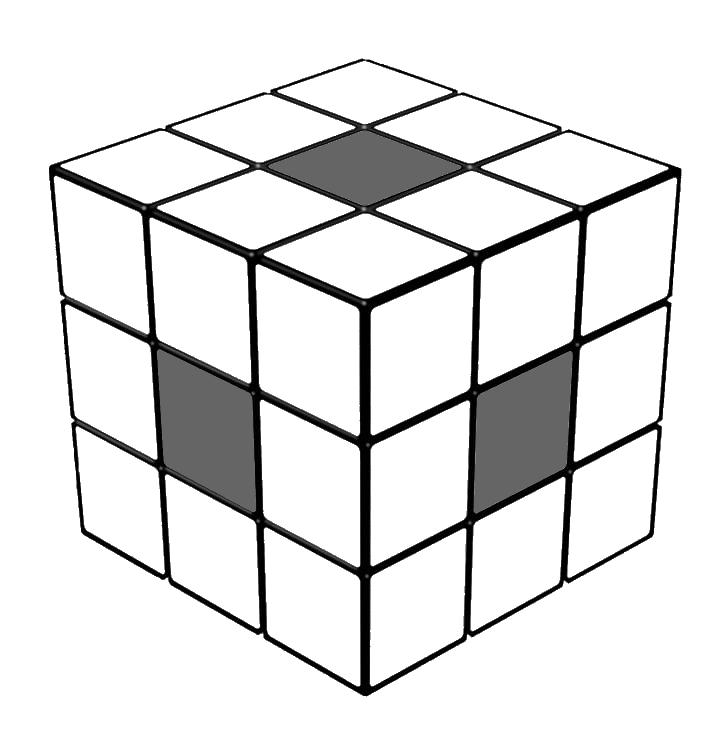
\includegraphics[height=2.5cm]{images/centri.png}
            \label{fig:centri}
        }
        \subfigure[ivice]{
            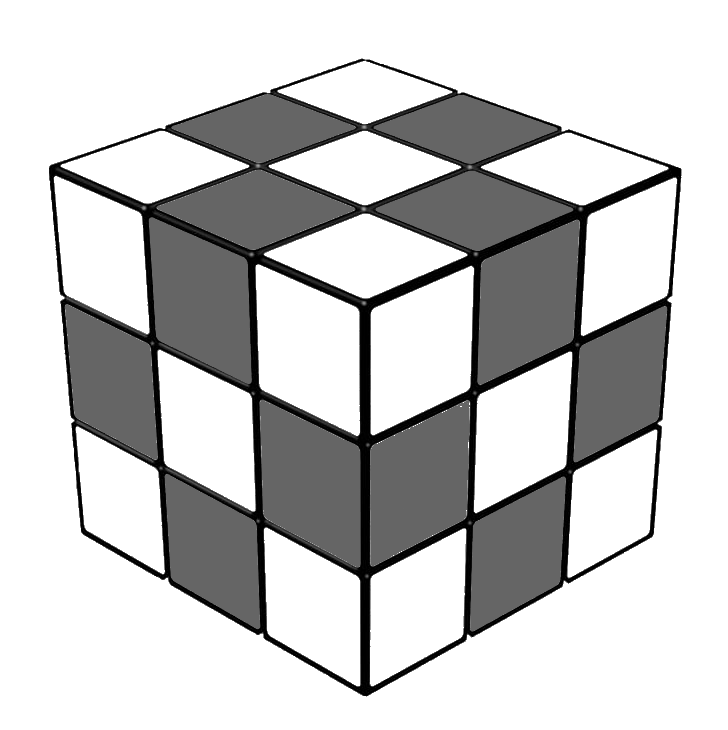
\includegraphics[height=2.5cm]{images/ivice.png}
            \label{fig:ivice}
        }
        \subfigure[ćoškovi]{
            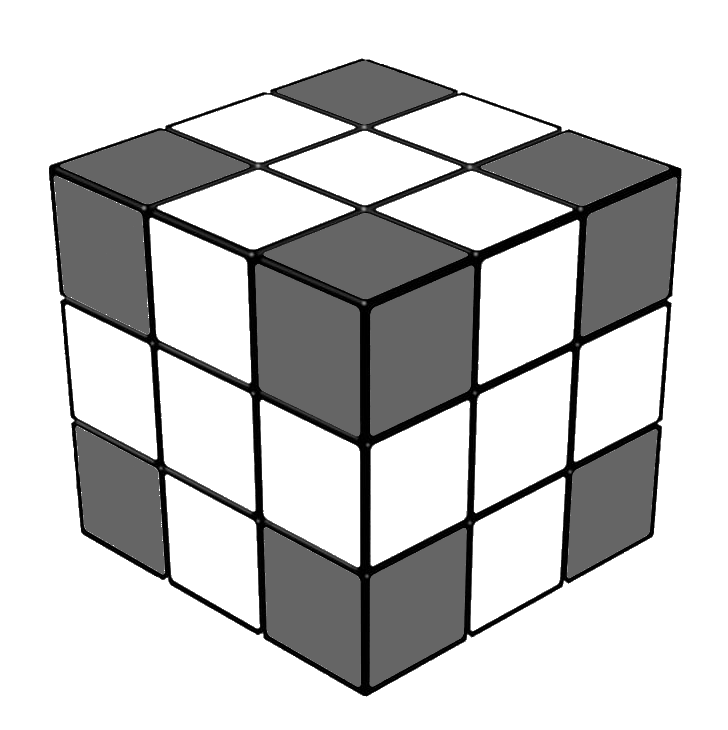
\includegraphics[height=2.5cm]{images/coskovi.png}
            \label{fig:coskovi}
        }
        \caption{}
        \label{fig:kockice}
    \end{figure}
    
\begin{itemize}
\item Među kockicama postoje one koje su obojene samo jednom bojom.
    One se nalaze u centru svake strane kocke i na njih dozvoljeni potezi ne utiču tj. ostavljaju ih na istom mestu (dozvoljeni potezi su opisani u narednom odeljku).
    Tih kockica ima 6 i zovemo ih \textit{centri} (slika \ref{fig:centri}). One nisu od tolikog značaja zato što su kod standardne Rubikove kocke praktichno fiksne\footnote{postoje varijacije Rubikove kocke gde se na stranama, umesto jednobojnih, nalaze šarene slike i onda centri dobijaju na značaju jer je za slaganje bitna njihova orijentacija}.
\item Druga grupa kockica je ona koja ima po dve svoje strane obojene.
    Takvih kockica ima 12 i dalje ih zovemo \textit{ivice} (engl. ~{\em edges}) (slika \ref{fig:ivice}).
\item Poslednja, treća grupa je ona sa po tri obojene strane kojih ima 8 i njih zovemo \textit{ćoškovi} (engl. ~{\em corners}) (slika \ref{fig:coskovi}).
\end{itemize} 


\section{Potezi}	
\label{sec:potezi}

Rubikova kocka ima 6 strana. Svaka od tih strana se može okretati i kocka se, različitim transformacijama, može dovesti u pozamašan broj različitih stanja. Međutim, najbitnije je opisati načine na koje se to može učiniti. Naime, svaka strana se može okrenuti za proizvoljan ugao, s tim što će okretanje za 360 stepeni vratiti kocku u stanje iz kojeg smo krenuli. Okretanje strane za ugao koji nije deljiv sa 90 će narušiti formu kocke. Stoga je najbitnije razmatrati samo one pomeraje strane koji su manji od 360 stepeni, a u isto vreme deljivi sa 90, odnosno 90, 180 i 270 stepeni. Kako se, dakle, jedna strana može pomeriti na samo 3 načina, zaključujemo da se na kocku možem primeniti 18 različitih poteza.

Kako su potezi uslovljeni pomerajima strana, za njih su uvedene oznake. Prihvaćeno je da se strana ispred nas označava sa F (engl. ~{\em front}), strana naspram nje (zadnja strana kocke) sa B (engl. ~{\em back}), desna strana sa R (engl. ~{\em right}), leva sa L (engl. ~{\em left}), dok se gornja i donja strana označavaju redom sa U (engl. ~{\em up}) i sa D (engl. ~{\em down}) (slika \ref{fig:stranekocke}).

\begin{figure}
        \centering\includegraphics[height=3cm]{images/kocka-strane.png} 
        \caption{}
        \label{fig:stranekocke}
\end{figure}

Dalje, sa S1, S2 i S' se označavaju redom pomeraji strana za 90, 180, odnosno 270 stepeni u smeru kazaljke na satu, ili matematički negativnom smeru. Na primer, R' bi značilo da se desna strana pomera za 270 stepeni u smeru kazaljke na satu ili za 90 stepeni u suprotnom smeru (zbog toga se taj pomeraj označava sa S', a ne sa S3).

Za samo rešenje kocke je potrebno definisati šta se to tačno smatra jednim potezom. Prirodno se nameće rešenje u kojem se za poteze S1 i S' uzima da su dužine 1, dok bi se za potez S2 smatralo da je dužine 2, jer se u suštini sastoji od dva poteza dužine 1. Međutim, ovakav pristup nije pogodan za traženje i određivanje algoritama za rešenje kocke. Stoga je kao standard prihvaćena \emph{metrika polovine okreta} (engl. ~{\em Half turn metric - HTM}). To znači da se svaki od 18 poteza, bilo da se sastoji od jednog ili dva okreta strane, smatra kao jedan. Prvi pomenuti način, onaj koji samo pomeraje za 90 stepeni smatra za poteze, naziva se \emph{metrika četvrtine poteza} (engl. ~{\em Quarter turn metric - QTM}). 

Nalaženje Božijeg broja u velikoj meri zavisi od toga koji od ova dva načina koristimo. Naime, kao što je već spomenuto, metrika polovine okreta je pogodnija za traženje algoritma rešavanja, pa je tako i nalaženje Božijeg broja za ovaj način bilo čak četiri godine brže i on iznosi 20. Tek 2014. godine je dokazano da je pri korišćenju metrike četvrtine okreta Božiji broj 26.

\section{Permutacije}
\label{permutacije}

Permutacije i orijentacije kockica su osobine koje određuju poziciju kockica, odnosno i samo stanje cele kocke.
Posmatrajmo sada ivice kocke i, konkretno, fiksirajmo jednu od njih (slika \ref{fig:ivica-pomeranje}). Kojim god pomerajem da promenimo mesto te ivice, ona će i dalje ostati ivica, ondosno, ivica pomeranjem ne može preći u neku drugu vrstu kockica, na primer u ćoškove, a isto važi i obrnuto, odnosno da nijedan ćošak pomerajem ne može postati ivica.
-
\begin{figure}[h]
        \centering
        \subfigure{
             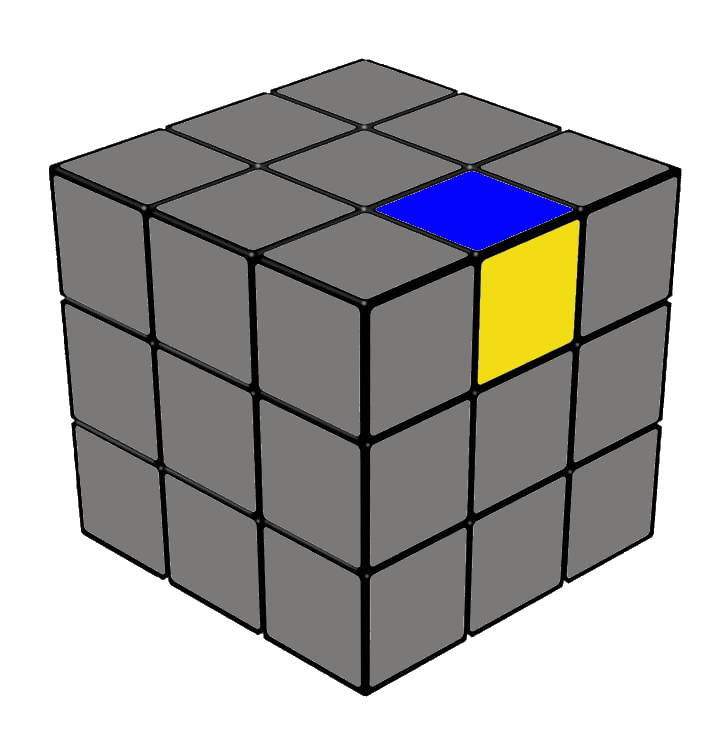
\includegraphics[height=2cm]{images/slozena-ivica.png}
        }
        \subfigure{
            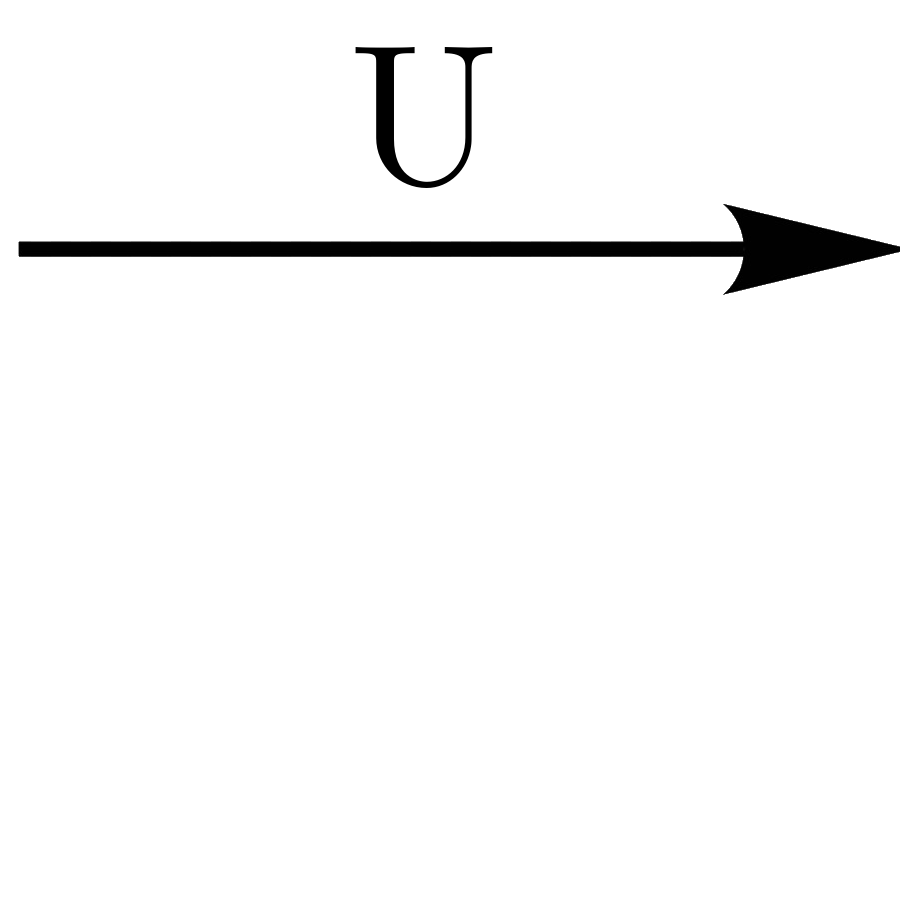
\includegraphics[height=1.5cm]{images/Uarrow.png} 
        }
        \subfigure{
             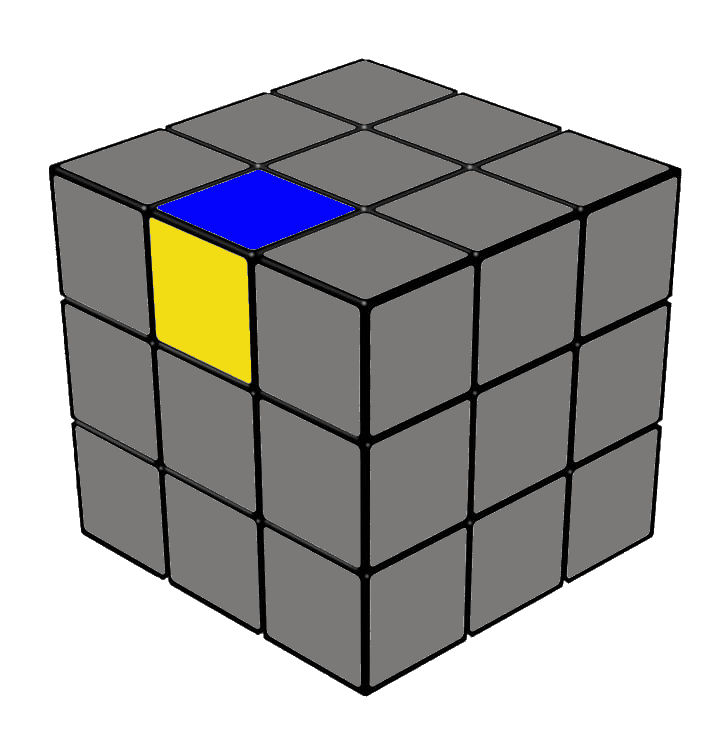
\includegraphics[height=2cm]{images/U-ivica.png}
        }
        \subfigure{
            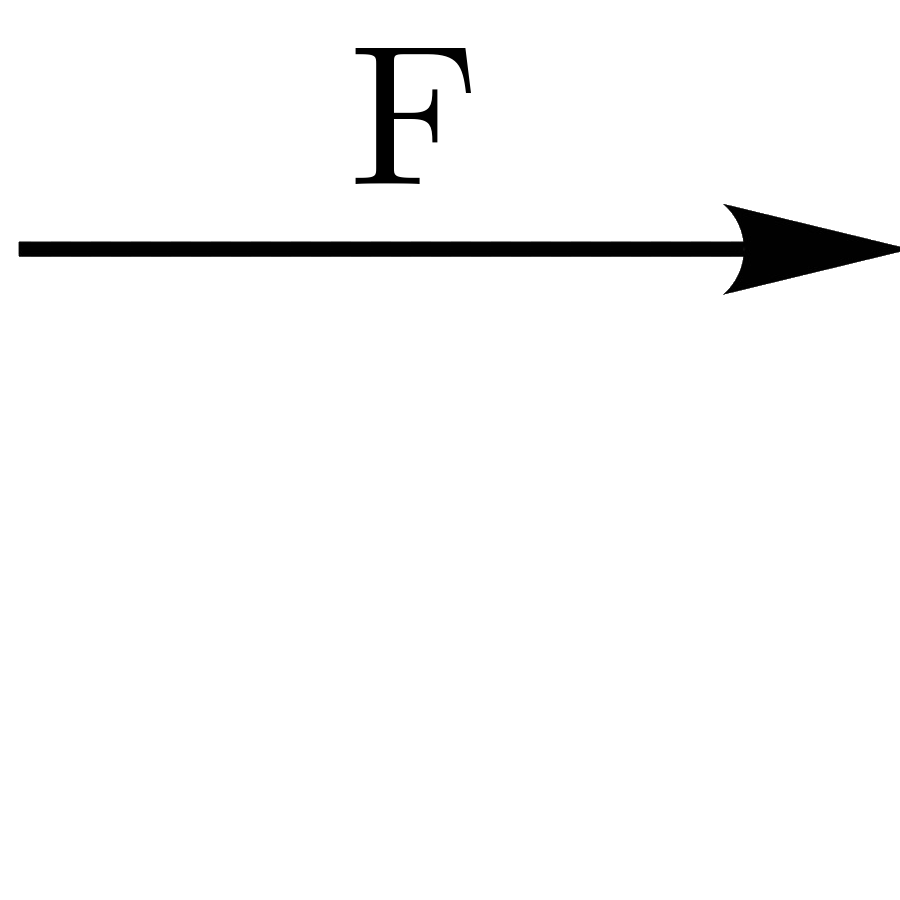
\includegraphics[height=1.5cm]{images/Farrow.png} 
        }
        \subfigure{
             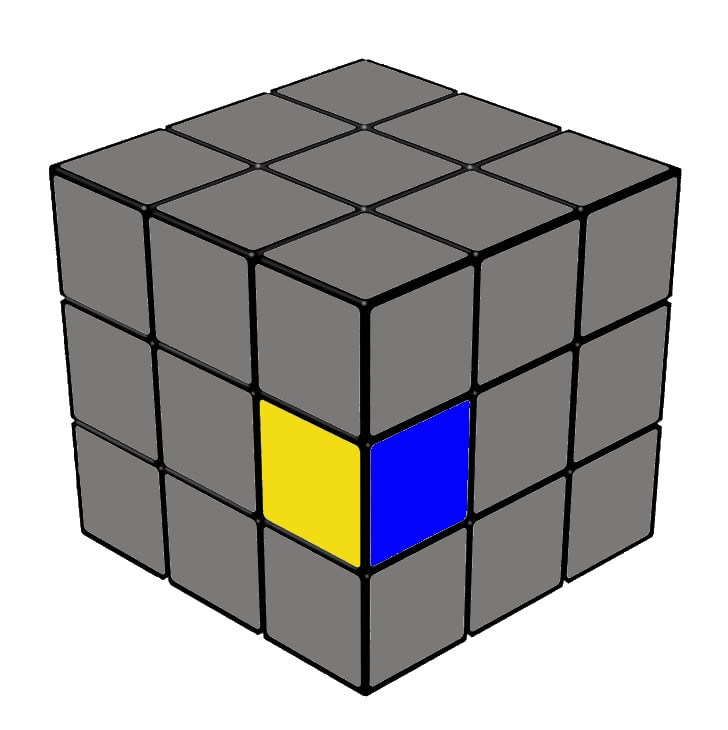
\includegraphics[height=2cm]{images/F-ivica.png}
        }
        \caption{}
        \label{fig:ivica-pomeranje}
    \end{figure}

Zato ivice imaju samo 12 mesta na kojima se mogu naći i jedno stanje kocke može imati samo jednu permutaciju tih ivica. S obzirom da se ivice i ćoškovi razlikuju i njihove permutacije se gledaju odvojeno jedne od drugih.

Ivice kocke se obeležavaju sa XY, gde su X i Y strane koje tu ivicu dele u složenoj kocki. Na primer, ivicu UR u složenoj kocki dele gornja (U) i desna (R) strana. Upravo zbog tog poređenja sa složenom kockom, ivica XY će uvek ostati XY, odnosno njena oznaka se potezima neće promeniti, na kojem god ona mestu završila.

Analogno ivicama, ćoškovi se obeležavaju sa XYZ, gde su X,Y i Z strane koje taj ćošak dele u složenoj kocki. Na primer, kao i kod ivica, gde su ivicu UR delile gornja i desna strana, tako će ćošak URF deliti gornja (U), desna (R) i prednja (F) strana. Baš kao i kod ivica, zbog toga što naziv ćoška zavisi od složene kocke, taj naziv se nikada ne može promeniti.

Nakon obeležavanja ivica i ćoškova stvara se novi problem. Primetimo da oznaka jednog ćoška, na primer URF, može da nam kaže koje strane ga dele, međutim ne može nam reći da li su boje raspoređene na onaj način kakav je potreban da bi se kocka složila. Baš iz tog razloga uveden je pojam \emph{orijentacije} ćoškova, odnosno ivica (slika \ref{fig:cosak-orijentacija-primer}).

Primetimo da, zbog broja strana koje ih dele, ivice mogu imati dve orijentacije, a ćoškovi tri. Te orijentacije obeležene su sa 0 i 1, kada se radi o ivicama, odnosno 0, 1 i 2 kada se radi o ćoškovima. Za orijentaciju 0 uzima se orijentacija ivica i ćoškova složene kocke. 

\begin{figure}[h]
        \centering
        \subfigure{
            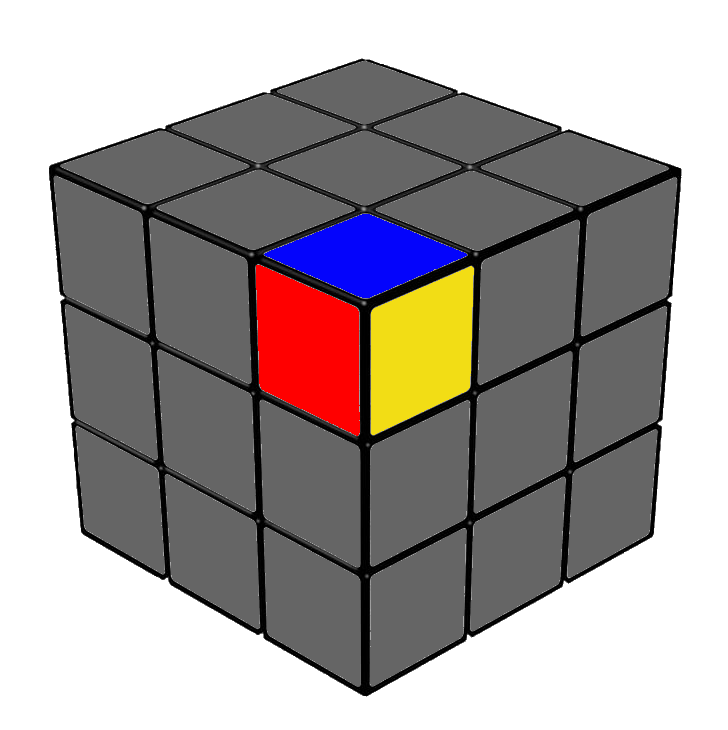
\includegraphics[height=2cm]{images/cosak-orijentacija-primer0.png}
        }
        \subfigure{
            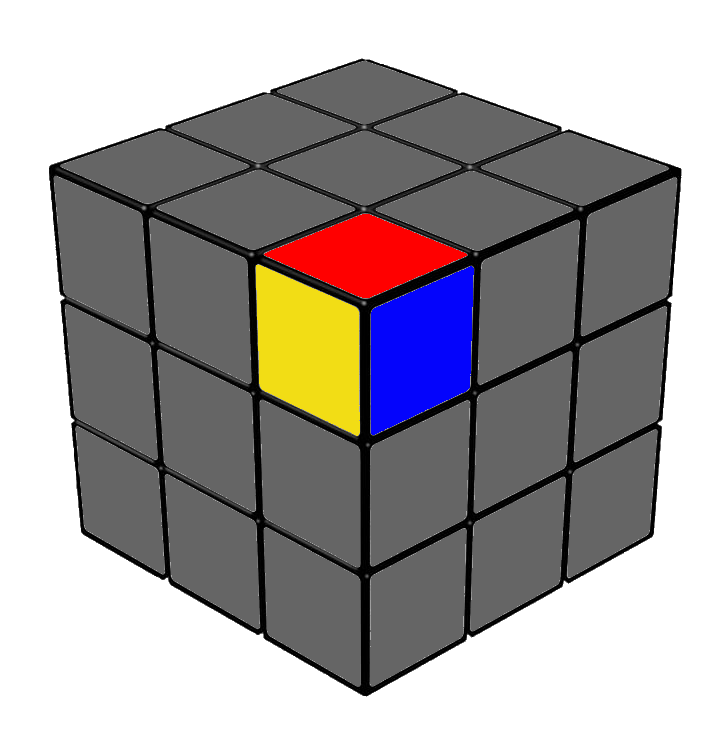
\includegraphics[height=2cm]{images/cosak-orijentacija-primer1.png}
        }
        \subfigure{
            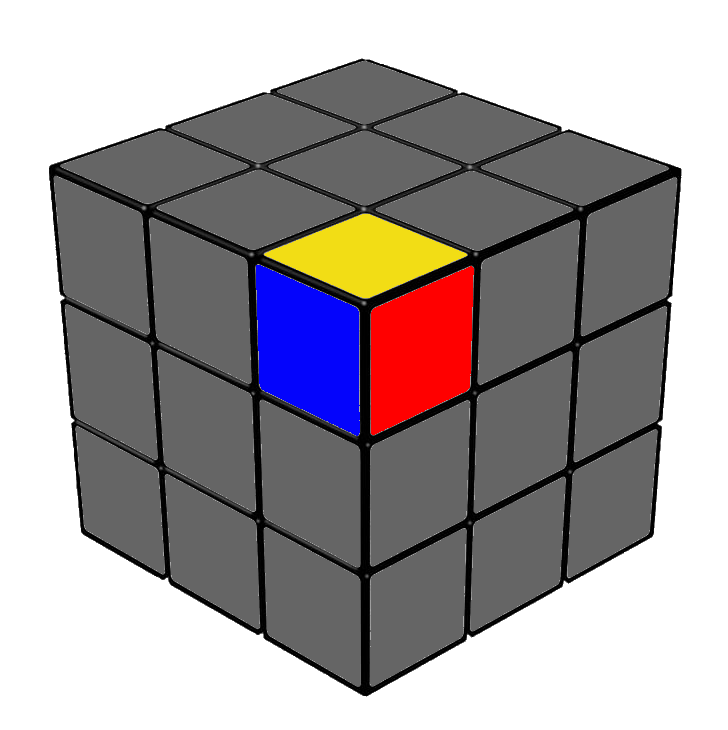
\includegraphics[height=2cm]{images/cosak-orijentacija-primer2.png}
        }
        \caption{\emph{Ćošak je na istom mestu ali drugačije orijentisan}}
        \label{fig:cosak-orijentacija-primer}
    \end{figure}



Sada možemo zaključiti da je svaka pozicija kocke precizno određena sa četiri koordinate: \textbf{permutacija ivica}, \textbf{orijentacija ivica}, \textbf{permutacija ćoškova} i \textbf{orijentacija ćoškova}.

Ivica ima 12, pa je broj njihovih permutacija jednak $12! = 479 001 600$. Za svaku od njih postoje dve orijentacij, međutim orijentacija poslednje je određena orijentacijom prethodnih 11 (ukoliko se 11 ivica složi na željeni način, 12. ivica će biti takođe složena; to se može zaključiti na primeru složene kocke, gde je nemoguće da samo jedna ivica bude pogrešno orijentisana), pa je broj mogućih orijentacija jednak $2^{11} = 2048$.

Čoškova ima 8, pa je broj njihovih permutacija jednak $8! = 40320$. Za razliku od orijentacija ivice, orijentacija jednog ćoška ima tri, ali, na isti način kao kod ivica, orijentacija poslednjeg ćoška je određena orijentacijama prethodnih 7. Stoga, broj orijentacija ćoškova je $3^{7} = 2187$

\begin{teorema} Permutacije svih kockica su parne.
\end{teorema}
\begin{proof}
    Posmatrajmo šta se dešava kada se jedna strana pomeri za 90 stepeni. Taj potez utiče na 4 ćoška i 4 ivice, i to tako što će svaki od njih zameniti mesta sa jednim susedom, odnosno desiće se 3 razmene ivica i 3 razmene ćoškova (prvi će se zameniti sa drugim, drugi sa trećim i treći sa četvrtim), pa se dobija da se jednim potezom desi 6 razmena, odnosno da je permutacija parna.
\end{proof}

Koliko pozicija može imati jedna kocka? Iz onoga što smo do sada videli, možemo zaključiti da postoji $12! \cdot 8!$ permutacija, međutim, zbog teoreme 1, znamo da one mogu biti samo parne. Zato je ukupan broj permutacija zapravo jednak $\frac{12! \cdot 8!}{2}$. Za svaku od tih permutacija postoji $2^{11} \cdot 3^{7}$ orijentacija (jer su one određene sa 11 ivica i 7 ćoškova), što znači da jedna kocka može imati $\frac{1}{2} \cdot 12! \cdot 8! \cdot 2^{11} \cdot 3^7 = 43,252,003,274,489,856,000$ različitih pozicija. Red veličine ove vrednosti je $10^{19}$ i to je jedan od glavnih razloga zašto je pronalazak algoritma za rešavanje bio toliki problem.

\begin{primer} I tabele treba da budu u svom okruženju, i na njih je neophodno referisati se u tekstu. Na primer, u tabeli \ref{tab:tabela1} su prikazana različita poravnanja u tabelama.

\begin{table}[h!]
\begin{center}
\caption{Razlčita poravnanja u okviru iste tabele ne treba koristiti jer su nepregledna.}
\begin{tabular}{|c|l|r|} \hline
centralno poravnanje& levo poravnanje& desno poravnanje\\ \hline
a &b&c\\ \hline
d &e&f\\ \hline
\end{tabular}
\label{tab:tabela1}
\end{center}
\end{table}

\end{primer}

\section{Algoritmi}
\label{sec:algoritmi}

\section{Zaključak}
\label{sec:zakljucak}

Ovde pišem zaključak. 
Ovde pišem zaključak. 
Ovde pišem zaključak. 
Ovde pišem zaključak. 
Ovde pišem zaključak. 
Ovde pišem zaključak. 
Ovde pišem zaključak. 
Ovde pišem zaključak. 
Ovde pišem zaključak. 
Ovde pišem zaključak. 
Ovde pišem zaključak. 
Ovde pišem zaključak. 


\addcontentsline{toc}{section}{Literatura}
\appendix

\iffalse
\bibliography{seminarski} 
\bibliographystyle{plain}
\fi

\begin{thebibliography}{9}

\bibitem{laski2009software} J. Laski and W. Stanley. \emph{Software Verification and Analysis}. Springer- Verlag, London, 2009.

\bibitem{gcc} Free Software Foundation. GNU gcc, 2013. on-line at: http://gcc. gnu.org/.

\bibitem{haltingproblem} A. M. Turing. \emph{On Computable Numbers, with an application to the Entscheidungsproblem}. Proceedings of the London Mathematical Society, 2(42):230–265, 1936.


\end{thebibliography}


\appendix
\section{Dodatak}
Ovde pišem dodatne stvari, ukoliko za time ima potrebe.
Ovde pišem dodatne stvari, ukoliko za time ima potrebe.
Ovde pišem dodatne stvari, ukoliko za time ima potrebe.
Ovde pišem dodatne stvari, ukoliko za time ima potrebe.
Ovde pišem dodatne stvari, ukoliko za time ima potrebe.


\end{document}
